
\chapter{Appendix}
\newpage

\section{User manual}
This section is dedicated to explain most common actions presented in the system. In the following points it will explained this information:

\begin{itemize}
\item How to reboot the full system.
\item How to manage MongoDB.
\item How to access remotely to the system.
\end{itemize}

Also, it will be explained more details we consider which are important in the system.\\

\subsection{How to reboot the full system}

A completely reboot should be likely established. For that purpose, we need to consider we have different subsystems that can lead to executing problems in the full system. Those subsystems are the following.

\begin{itemize}
\item Network system.
\item Database system.
\item Sensor system.
\item Computing system.
\end{itemize}

In the following section how to manage with this systems and operation is explained.\\

\subsubsection{Restart network system}

At first, we are using a system which manages heavy information. In some situations, the system should support a higher number of petitions to queries to the database or intensive transmission of information that can generates failures in the network architecture.\\

In this case, a restart of the whole network is sometimes required. To do it, it is necessary to know the different elements which composed each subsystem. The elements we have in our system are the following:

\begin{itemize}
\item Router.
\item Raspberry PI.
\item Different devices connected to the router.
\begin{itemize}
\item Smartphones.
\item Computer.
\item Sensors.
\end{itemize}	
\end{itemize}

The router is the network brain of our system due to it control all information related to the network. It will allow to stablish the among communication with all the devices of the system.\\

If we have to restart the network, the steps are:

\begin{itemize}
\item Press the power on button of the router.
\item Wait some seconds before plug in it again.
\item Press the power on button of the router again.
\item Wait two minutes until the devices are connected again to the router.
\end{itemize}

If everything is correct, the router will allow the communication between the different devices of the network again. As the configuration is done by the router, user does not have to care about the configuration of the different devices.\\

\subsubsection{Restart the database}

When a restart of the database is required, we need to control the Raspberry Pi which can be done following different options.

\begin{itemize}
\item Remote access to the Raspberry Pi.
\begin{itemize}
\item Via Linux terminal.
\item Via Mac terminal.
\item Via Putty. This software is available to download it, and it is really useful for Windows’ users.
\end{itemize}
\item Connecting peripherical devices to the Raspberry Pi.
\begin{itemize}
\item Monitor.
\item Keyboard.
\item Mouse (it is not mandatory but maybe it is useful to have one).
\end{itemize}
\end{itemize}

In the following sections it will be explained how to create a remote connection to the Raspberry Pi and how to access with different peripherical devices to the Raspberry Pi.\\

\subsubsection{Restart the sensor system and the Raspberry PI}

This is the most common way to restart the system. Usually, it is only needed to restart the Raspberry Pi with the Arduino which is connected to the Raspberry Pi.\\

To do it, next, it is required to follow these steps.

\begin{enumerate}

\item Disconnect the Raspberry Pi from the current.
\item Disconnect the Arduino from the Raspberry Pi.
\item Wait some seconds.
\item Connect again the Arduino to the Raspberry Pi.
\item Plug in the current of the Raspberry Pi.
\item Wait two minutes until the Raspberry Pi finishes its booting operations.

\end{enumerate}

After applying these steps, we ensure the system has been reset.\\

\subsection{How to manage MongoDB}

To manage databases, it is required to know the status of them. MongoDB is a database system which allows us to store different kind of information. In this section, it will be explained how to know different information about our MongoDB database system.

\subsubsection{See the current version of MongoDB}

In case we a working with a \textit{Linux} system, the steps after opening a terminal are:

\textit{sudo mongod –version}\\

This command will show the current version used by MongoDB. This operation is useful to know which \textit{API}\cite{what_is_an_API} (\textit{Application Programming Interface}) to use to store, query or maintain the different information we have stored in our database.\\

It is recommended to use MongoDB version up to 2.6. If we are under 2.6 version, it is recommended to update it to 2.6 or greater versions.

\subsubsection{Check mongod service}

In case the system suffers a problem related to a restart or a power off of our system, the services can go down. This is typically a problem we have when we are managing Information Systems.\\

If we need to check if our MongoDB database system is working, we need to follow these steps.

\begin{itemize}
\item Open a Linux terminal.
\item Get administrator privileges using \textit{sudo su}.
\item Run \textit{ps -ax | grep mongo}.
\end{itemize}

With these commands, it would be possible to see if MongoDB is running in our system. If we see something like the information described in the following image, it will mean MongoDB is running in our system.\\

\begin{figure}[H]
\begin{centering}
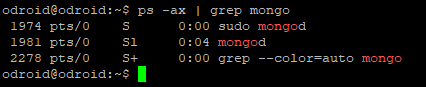
\includegraphics[scale=1]{IMGS/check_mongodb_is_running.PNG}
\caption{How to display MongoDB service when it is running \label{How to display MongoDB service when it is running}}
\end{centering}
\end{figure} 
 
As we can see in the picture displayed before, there are some services running with the name \textbf{mongo}. The last one is irrelevant for us, because it is the result obtained after executing \textit{ps -ax | grep mongo}. The information which is important for us is the different lines displayed before, \textit{sudo mongod and mongod}. These lines are telling us that MongoDB is running properly in our system.\\

The steps described the MongoDB status. There are several ways to check. For example, after the installation of MongoDB using the package manager of Linux, the system will create a new entire into \textit{/etc/init.d} and in services which will allow us to identify if the service is running. This entry is name as service. Linux has lot of services, and it is possible to query if there are services running in our machine.\\

If we have created a service entry in our system, it is possible to query the status of the service using sudo service [name of the service we want to query]. To know if MongoDB is running, we can type \textit{sudo service mongod status}. If the service is installed in our machine, it will be possible to see the following information.\\

\begin{figure}[H]
\begin{centering}
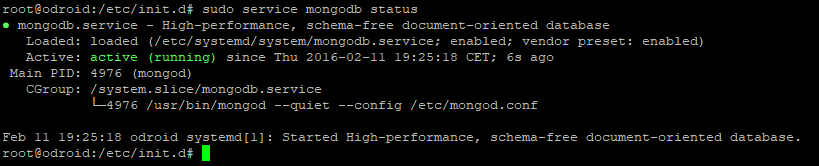
\includegraphics[scale=0.7]{IMGS/mongodb_status.PNG}
\caption{MongoDB's service is active \label{MongoDB's service is active}}
\end{centering}
\end{figure} 
 
To display this information, it is needed to type in the Linux console \textit{sudo service mongodb status}.\\

As can be seen, the server is running, showing its \textit{pid} (identification associated to MongoDB’s thread) and its executable (allocated in \textit{/usr/bin/mongod}).\\

\subsubsection{Start MongoDB service}

This operation is usually useful when there is a problem on the system (for example, MongoDB has not started at the beginning of the booting process) or when there is no configuration to run it automatically.\\

To do it, it is necessary to type in the console \textit{sudo service mongodb start}. With this command we will tell \textit{mongodb} it has to run.\\

\begin{figure}[H]
\begin{centering}
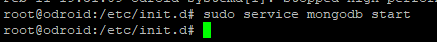
\includegraphics[scale=1]{IMGS/start_mongodb_service.PNG}
\caption{Start MongoDB's service \label{Start MongoDB's service}}
\end{centering}
\end{figure}
 
To check if MongoDB is running, it is necessary to type \textit{sudo service mongod status}. If we noticed the system running after executing this command, we do not have to be worried about the startup of the service.

\subsubsection{Stop MongoDB service}

Sometimes, it is not only need to start the daemon process. There are several situations where we want to stop the database server, for example, if there is a query that has blocked the database. In these cases, it is useful to have control of MongoDB’s service.\\

To do it, we just only need to type \textit{sudo service mongod stop}. It is useful to check if the service has stopped or not. To do it, we just have to type \textit{sudo service mongod status}. If we see some information like not running, then we can ensure the service has stopped properly.\\

In the following picture there is an example of the execution of this last command.

\begin{figure}[H]
\begin{centering}
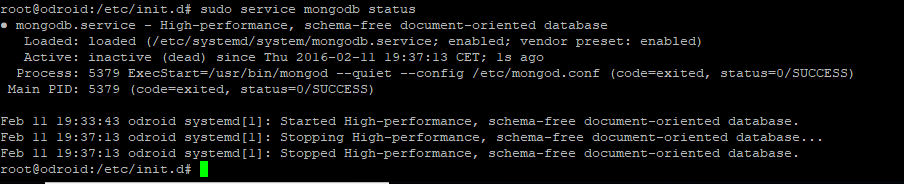
\includegraphics[scale=0.65]{IMGS/stop_mongodb_service.PNG}
\caption{Stop MongoDB's service \label{Stop MongoDB's service}}
\end{centering}
\end{figure}

\subsubsection{How to manage MongoDB with no services installed in the system}

In some situations, it is possible to see that MongoDB has not a service architecture defined.\\

When there is an installation process in Linux, the system will create different link files, executable files and configuration files. Some of the files created in the installation process will be copied to the folder \textit{/usr} and the files related to configurations will be placed in \textit{/etc}.\\

MongoDB will create all the configuration files in \textit{/etc}. Here, it is possible to define the different parameters needed to start running the system like:

\begin{itemize}

\item Path of the executable file to start the database system.

\item Path of the different log files where it is possible to see the debugging status of the database system or problems related to configuration.

\item Path of the folder which is going to be used to store the different databases used by MongoDB.

\item Configuration of the user.

\item Configuration of the listen port used by MongoDB. This port is used to allow possible incoming connections to the database.

\item Mode of execution of MongoDB. The different modes we have available are the following:

\begin{itemize}

\item Verbose mode. This mode allows the user to see the output generated by the full system. It is possible to see the incoming connections, problems occurred during the execution of the database system, timeouts, logouts, logins, etc.

\item Silent mode. This mode does not display information about the execution of the database system. This is the default mode used by the main program.

\end{itemize}

\item Configuration used to authenticate the different user connected to the database.

\item Allowed IP addresses to access to the database.

\end{itemize}

All this information is stored in \textit{/etc} in one file named \textbf{mongod.conf}. It is possible to edit this file if it is needed to do it, but it is necessary to be careful if we apply any modifications because it is possible after those modifications the system will not run correctly.\\

There is another important folder that is needed to mention in this section. This folder is \textit{init.d} and it is stored in \textit{/etc}. This folder will contain all the different executable shell scripts needed by the system. Obviously, MongoDB will create some files in this folder. The most important file to consider is \textit{mongodb}. It is possible to control all the operations done by MongoDB with this file. The possible operations are start, stop, restart and display status. Those operations are executed as follows.

\begin{itemize}

\item Type in the console \textit{sudo /etc/init.d/mongodb start} to start MongoDB. After the execution of this command, MongoDB must run in the background.

\item Type in the console \textit{sudo /etc/init.d/mongodb stop} to stop MongoDB. This command does the same operations described in the service section of MongoDB.

\item Type in the console \textit{sudo /etc/init.d/mongodb restart} to restart MongoDB.

\item Type \textit{sudo /etc/init.d/mongodb status} to show the status of MongoDB. The information displayed will exactly the same if we execute \textit{sudo service mongod status}.

\end{itemize}

This knowledge is required to manage a MongoDB database system.\\

It is important to know that all the commands described in this section needs the sentence \textit{sudo}. In all Linux system, if the user wants to modify some features related to configuration of some programs, it is needed to use it. This capability allows to control the access to certain files of folder that could be damaged by some users.

\subsubsection{Check MongoDB network connection}

As it was explained before, sometimes it is necessary to check if MongoDB is running in the system or, for example, to reboot it in case we have problems when we are storing information in our database. In some cases, MongoDB is running although it is not possible to access the databases. The common reason is the rejection of incoming connections. When we have this problem, it is necessary to check if MongoDB has its port reachable. To do it, it is necessary to execute the following command.\\

\textit{sudo netstat -l | grep 27017}\\

With this command, we will ask \textit{Raspbian} if there are any processes using this port. If it is not displayed any information after executing this command, then we can be ensured the system is not allowing incoming connections to the databases we have.\\

If we have this problem, then we should restart again MongoDB as it was explained as before.

\section{Solution to frequent problems}

This section of the user manual is dedicated to explain how to solve common problems we can find when we are working with MongoDB.\\

It is often to have problems related to network communication, storage or problems related to how to manage the MongoDB service installed in our machine.\\

In the following subsections it will be explained how to deal with all these problems.

\subsection{Remote access to Raspberry Pi}

As we explained before, there are several tools to allow remote access to the Raspberry Pi. The Raspberry Pi allows by default demote management, and this is one of the most powerful capabilities it has. Thanks to remote access we can manage the full system.\\

Then, it would be explained how to connect to Raspberry Pi using \textit{Putty} due to is the most extended protocol for remote connection for Windows' users.

To do it, first it is needed to download this software from its webpage, after we have downloaded it, we have to open \textbf{Putty}.\\

\begin{figure}[H]
\begin{centering}
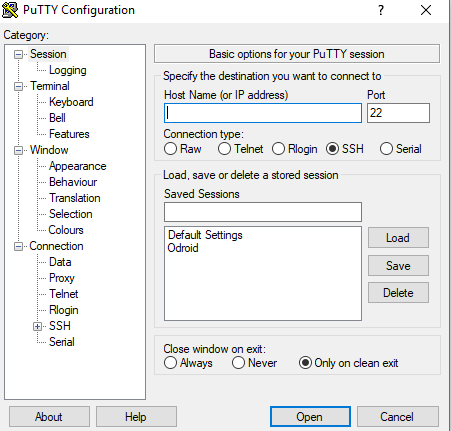
\includegraphics[scale=1]{IMGS/putty_interface.PNG}
\caption{Putty's interface \label{Putty's interface}}
\end{centering}
\end{figure} 
 
As it is possible to see in the picture, we have some fields we have to complete. The different fields we have are the following:

\begin{enumerate}

\item Host name or IP address. This field has to be fielded with the IP address used by the Raspberry PI. In our case, the IP address of our Raspberry Pi will have the structure \textit{192.168.1.X} (the X has to be replaced by the last number of the IP address used by the Raspberry PI). By default, the Raspberry Pi uses \textit{192.168.1.50}. If the user does not know the network address used by the Raspberry Pi, it is needed to read the section How to see Raspberry Pi’s network address.

\item Port. It is not needed to modify this port because the Raspberry Pi uses by default the port \textit{22} for \textbf{SSH} connections.

\end{enumerate}

After filling this information, we have to press Open. When we have pressed Open it will be displayed a console. This console will have the following structure.

\begin{figure}[H]
\begin{centering}
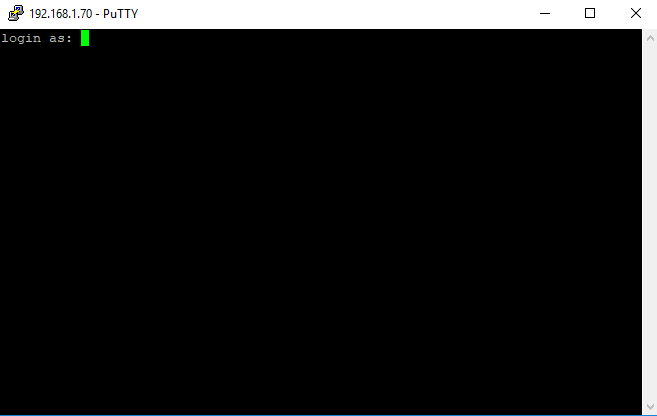
\includegraphics[scale=0.8]{IMGS/loggin_putty.PNG}
\caption{Loggin into Raspberry Pi \label{Loggin into Raspberry Pi}}
\end{centering}
\end{figure} 
 
Here, Raspberry Pi requires the username of the system. In this step we have to type \textit{pi} (it is important to type it in lowercase).\\

Next, Raspberry Pi will ask us about the password. In the following picture it will be displayed the information related to the password request.

\begin{figure}[H]
\begin{centering}
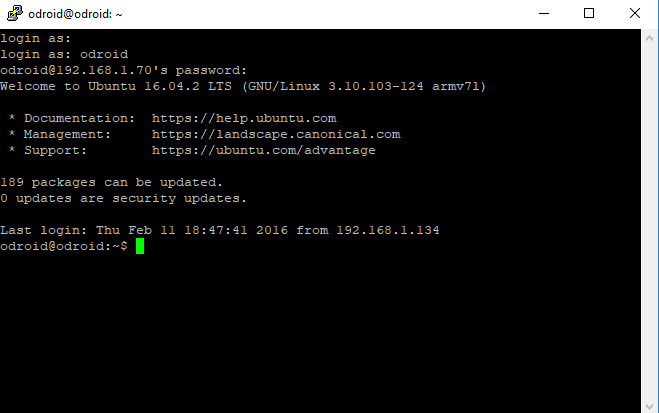
\includegraphics[scale=0.8]{IMGS/loggin_putty_pass.PNG}
\caption{Loggin into Raspberry Pi with its password \label{Loggin into Raspberry Pi with its password}}
\end{centering}
\end{figure}
 
Now we have to type raspberry (be careful with uppercase and lowercase), and the prompt of the system will be displayed.
To restart the database daemon, it is necessary to apply the different steps described in the section Check MongoDB’s status.

\subsection{Moving the measure system}

In some situations, it is necessary to turn off the full system because it is needed to do some hardware modifications. To do it, it is important to turn off the different components we have in our system to avoid electrical problems or storage problems (it is possible that after disconnecting some devices in our system, the MongoDB daemon could write corrupt information in the database we are using). To avoid these problems, it is important to do the following steps.

\begin{itemize}

\item Turn off the database. This step is not mandatory, but it is useful to know we could do it to be ensure that the daemon is not doing any important stuff. To do it, we need to execute the command:
\textit{sudo /etc/init.d/mongod stop}

\item Turn off the Raspberry PI. It is really important to do this step if we want to disconnect all the sensors or we want to move the full system. If we do not follow this step, it is possible we can break down the database which is being used by MongoDB or it is possible to generate wrong measures in our database. If we want to turn off the Raspberry PI, it is necessary to execute the command:
\textit{sudo shutdown now}

\item Disconnect the rest of the device from the electrical supply.

\end{itemize}

It is important to know that after doing reset explained before, it is necessary to fix the date of the system. This step must be done because our system does not have any connection to Internet to synchronize its date information with any Time Server. To do it, it is necessary to execute the following command.\\

\textit{sudo date -s 'YEAR-MONTH-DAY HOUR:MINUTES:SECONDS'}\\

An example of the execution of this command is for example:\\

\textit{sudo date -s '2018-05-25 18:40:10'}

\subsubsection{How to see Raspberry Pi’s network address}

In some cases, the user does not configure a static network address in the Raspberry Pi. Also, this configuration is missing and the Raspberry Pi has enabled \textit{DHCP} configuration. Due to this problem, the user has to look for the device in the network.\\

When this problem happens, it is possible to check the configuration with the following methods:

\begin{itemize}

\item Direct connection to Raspberry Pi. It is possible to have a direct connection to the Raspberry Pi using a monitor, a keyboard and a mouse. If we decide to use this solution, we need to follow these steps.

\begin{itemize}

\item Open a Linux terminal going directly to applications and after seeing Terminal.

\item When we have opened the Linux terminal, we have to type \textit{ifconfig} in the terminal. The information displayed in the screen is:

\begin{figure}[H]
\begin{centering}
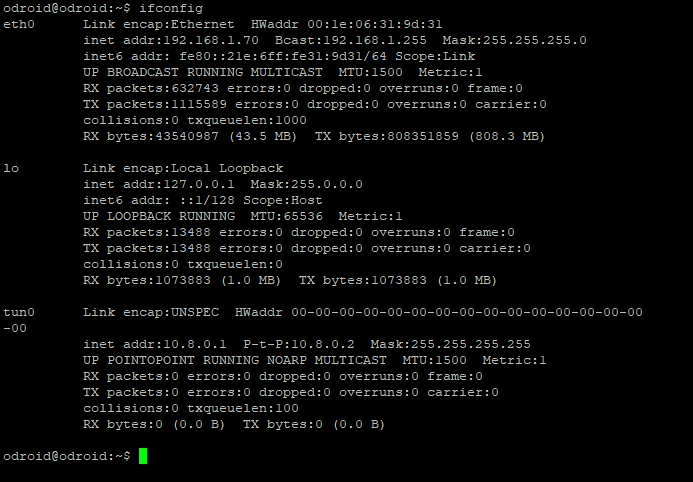
\includegraphics[scale=0.8]{IMGS/ifconfig_raspberry_pi.PNG}
\caption{Network adapters Raspberry Pi \label{Network adapters Raspberry Pi}}
\end{centering}
\end{figure} 

\item As it is possible to see, some information of the Raspberry Pi is shown.

\item Next, we need to change the IP address of the interface \textit{eth0}. In this interface it is possible to see its IP address (represented in the picture as \textit{inet addr: 192.168.1.X}). This IP address is the one used by the Raspberry Pi.

\item If the user does not know how to log in the Raspberry Pi, please read the section Remote access to Raspberry Pi.

\end{itemize}

\item Check the IP address using the router. This option is recommended if we can not connect to the Raspberry Pi. For that purpose, the next steps are required:

\begin{itemize}

\item Open a web browser (for example \textbf{Firefox}) and type in the address field \textbf{192.168.1.1}.

\begin{figure}[H]
\begin{centering}
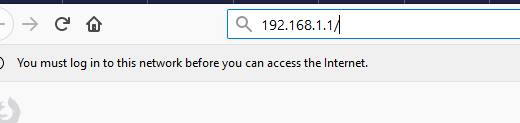
\includegraphics[scale=1]{IMGS/router_address.PNG}
\caption{IP address of the router \label{IP address of the router}}
\end{centering}
\end{figure} 

\item After entering in the address displayed in the pictured, it will be shown a login dialog. In the login dialog we need to enter user and the password of the router.

\begin{itemize}

\item User: \textit{admin} / Password: \textit{admin}
\item User: \textit{admin} / Password: \textit{1234}

\end{itemize}

\item After typing this information, we will see the information associated to the Raspberry Pi.

\end{itemize}

\end{itemize}

\subsubsection{How to proceed when the database is corrupt}

In case we want to move the system and we do not have knowledge about it, we can generate several problems in our database, as storage problems. When it happens, normally, \textbf{MongoDB} cannot run and we will see in \textbf{3TStudio} there are no new information in the database. When we have this problem, it is necessary to remove the corrupt information we have in our database. It is important to know that we will lose the information we have stored in our database.

\begin{enumerate}

\item The most important thing is that we need to stop MongoDB daemon. To do it we need to execute:

\begin{enumerate}

\item \textit{sudo /etc/init.d/mongod stop}

\end{enumerate}

\item We need to move to the folder where the database is saved. To do it, it is necessary to execute the following commands.

\begin{enumerate}

\item \textit{cd /home/pi}
\item \textit{cd databases}

\end{enumerate}

\item When we are in the database folder, we need to remove all the information related to the database which is corrupt. To do it, we need to execute.

\begin{enumerate}

\item \textit{sudo rm material*}

\end{enumerate}

\item When we have removed all the files related to the database which we were using before, we need to start again MongoDB daemon. To start again MongoDB daemon, we need to execute:

\begin{enumerate}

\item \textit{sudo /etc/init.d/mongod start}

\end{enumerate}

\item Wait until thirty seconds until the database is running and check if it is possible to connect to it using \textbf{3TStudio}.

\end{enumerate}

\section{Limits of the system}

In the following section it will be explained the different things we need to consider about our measure system. All these items should carefully consider if we want to do a new modification in the system.

\begin{enumerate}

\item If it is necessary to move the full system, it is important to disconnect the different components described in the points explained before.

\item To disconnect the different components we have in the measure system, follow the different tips we have explained before.

\item If it is necessary to modify or to replace some components in the system it is recommended to disconnect the system as it was explained before.

\item It is necessary to extract the information which is stored in the database periodically. The system can store up to \textit{\textbf{two Gigabytes}} of information.

\item Do not let the system to reach \textit{\textbf{two Gigabytes}} of information in the database. If it happens it is necessary to clean up the database and it will be lost the information stored.

\item If there is any problem in the communication to the Raspberry PI, be ensure that the service of the database is executing in the background.

\item If the Raspberry PI is disconnected from the supply, it is necessary to fix its date information. Remember it has not a Time Server to synchronize its date information.

\item The system has no Internet connection. If it is needed to modify something in the system it is recommended to create a Virtual Machine to download new packages.

\item If MongoDB is updated it is necessary to check the compatibility of new packages downloaded. Also, the API used to store the information in the Database.

\item In the future it is recommended to update MongoDB to a 64bits version. The 32bits version only allows you to store up to two Gigabytes of information. By default, \textit{Raspbian} packages install the 32Bits version in the system, so we have to be careful when we want to install MongoDB in our system.

\end{enumerate}

